\documentclass{article}

\usepackage{graphicx} % Required for inserting images
\usepackage[left=1in,right=1in,top=1in,bottom=1in]{geometry} \usepackage{amsmath}
\usepackage{amsthm} %proof environment
\usepackage{amsthm} %proof environment
\usepackage{amssymb}
\usepackage{amsfonts}
\usepackage{enumitem} %nice lists
\usepackage{verbatim} %useful for something 
\usepackage{xcolor}
\usepackage{setspace}
\usepackage{titlesec}
\usepackage{blindtext} % I have no idea what this is 
\usepackage{caption}  % need this for unnumbered captions/figures
\usepackage{natbib}
\usepackage{appendix}
\usepackage{tikz}
\usepackage{hyperref}


\hypersetup{
    colorlinks=true,
    linkcolor=blue,
    filecolor=magenta,      
    urlcolor=blue,
    pdftitle={Overleaf Example},
    pdfpagemode=FullScreen,
    }

\titleformat{\section}{\bfseries\Large}{Problem \thesection:}{5pt}{}

\begin{document}

\title{AM 216 - Stochastic Differential Equations: Assignment 1}
\author{Dante Buhl}


\newcommand{\wrms}{w_{\text{rms}}}
\newcommand{\bs}[1]{\boldsymbol{#1}}
\newcommand{\tb}[1]{\textbf{#1}}
\newcommand{\bmp}[1]{\begin{minipage}{#1\textwidth}}
\newcommand{\emp}{\end{minipage}}
\newcommand{\R}{\mathbb{R}}
\newcommand{\C}{\mathbb{C}}
\newcommand{\N}{\mathcal{N}}
\newcommand{\Var}{\text{Var}}
\newcommand{\Cov}{\text{Cov}}
\newcommand{\Bino}{\text{Bino}}
\newcommand{\Norm}{\mathcal{N}}
\newcommand{\erf}{\text{erf}}
%\newcommand{\K}{\bs{\mathrm{K}}}
\newcommand{\m}{\bs{\mu}_*}
\newcommand{\s}{\bs{\Sigma}_*}
\newcommand{\dt}{\Delta t}
\newcommand{\dx}{\Delta x}
\newcommand{\tr}[1]{\text{Tr}(#1)}
\newcommand{\Tr}[1]{\text{Tr}(#1)}
\newcommand{\Div}{\nabla \cdot}
\renewcommand{\div}{\nabla \cdot}
\newcommand{\Curl}{\nabla \times}
\newcommand{\Grad}{\nabla}
\newcommand{\grad}{\nabla}
\newcommand{\grads}{\nabla_s}
\newcommand{\gradf}{\nabla_f}
\newcommand{\xs}{x_s}
\newcommand{\x}{\bs{x}}
\newcommand{\xf}{x_f}
\newcommand{\ts}{t_s}
\newcommand{\tf}{t_f}
\newcommand{\pt}{\partial t}
\newcommand{\pz}{\partial z}
\newcommand{\uvec}{\bs{u}}
\newcommand{\bvec}{\bs{B}}
\newcommand{\nvec}{\hat{\bs{n}}}
\newcommand{\tu}{\tilde{\uvec}}
\newcommand{\B}{\bs{B}}
\newcommand{\A}{\bs{A}}
\newcommand{\jvec}{\bs{j}}
\newcommand{\F}{\bs{F}}
\newcommand{\T}{\tilde{T}}
\newcommand{\ez}{\bs{e}_z}
\newcommand{\ex}{\bs{e}_x}
\newcommand{\ey}{\bs{e}_y}
\newcommand{\eo}{\bs{e}_{\bs{\Omega}}}
\newcommand{\ppt}[1]{\frac{\partial #1}{\partial t}}
\newcommand{\pp}[2]{\frac{\partial #1}{\partial #2}}
\newcommand{\pptwo}[2]{\frac{\partial^2 #1}{\partial #2^2}}
\newcommand{\ddtwo}[2]{\frac{d^2 #1}{d #2^2}}
\newcommand{\DDt}[1]{\frac{D #1}{D t}}
\newcommand{\ppts}[1]{\frac{\partial #1}{\partial t_s}}
\newcommand{\pptf}[1]{\frac{\partial #1}{\partial t_f}}
\newcommand{\ppz}[1]{\frac{\partial #1}{\partial z}}
\newcommand{\ddz}[1]{\frac{d #1}{d z}}
\newcommand{\ppzetas}[1]{\frac{\partial^2 #1}{\partial \zeta^2}}
\newcommand{\ppzs}[1]{\frac{\partial #1}{\partial z_s}}
\newcommand{\ppzf}[1]{\frac{\partial #1}{\partial z_f}}
\newcommand{\ppx}[1]{\frac{\partial #1}{\partial x}}
\newcommand{\ddx}[1]{\frac{d #1}{d x}}
\newcommand{\ppxi}[1]{\frac{\partial #1}{\partial x_i}}
\newcommand{\ppxj}[1]{\frac{\partial #1}{\partial x_j}}
\newcommand{\ppy}[1]{\frac{\partial #1}{\partial y}}
\newcommand{\ppzeta}[1]{\frac{\partial #1}{\partial \zeta}}
\renewcommand{\k}{\bs{k}}
\newcommand{\real}[1]{\text{Re}\left[#1\right]}


\maketitle 
% This line removes the automatic indentation on new paragraphs
\setlength{\parindent}{0pt}

\section{Two Dice}
Roll a set of two fair 6-sided dice, one colored red the other white. Assume that the two dice
roll independently. Record the two numbers facing up as $X_1$ and $X_2$.

%\begin{enumerate}[label=\alph*]
\begin{enumerate}[label=\roman*)]
    \item  Mathematically describe the format of outcome. Describe the sample space.
        \begin{proof}
            The two quantities $X_1$ and $X_2$ are samples from a given discrete
            probability distribution. The sample space has six equally likely
            outcomes ${1, 2, 3, 4, 5, 6}$ with an expected value of $E(X) =
            3.5$. The two samples $X_1$ and $X_2$ are independent and
            identically distributed samples. 
        \end{proof}
    \item Let $X$ be the absolute difference between $X_1$ and $X_2$. Is $X$ a random variable?
        \begin{proof}
            Yes, the sum/difference of two random variables is also a random
            variable, albeit with a different sample space and expected value.
            We can exam the sample space to find that there are 6 possibilities
            of different likelihood: $S = {0, 1, 2, 3, 4, 5}$, with 5 being the
            least likely (only two outcomes where the result is 5) and 1 being
            the most likely (there are ten outcomes with a result of 1).
        \end{proof}
    \item Find the PMF of $X$, $E(X)$
        \begin{proof}
            Specifically, 
            \begin{center}
            \begin{tabular}{||c c||} 
                \hline
                k & P(X = k)\\ [0.5ex] 
                \hline\hline
                0 & 0.166... \\ 
                \hline
                1 & 0.277... \\ 
                \hline
                2 & 0.222... \\
                \hline
                3 & 0.166... \\
                \hline
                4 & 0.111... \\
                \hline
                5 & 0.055... \\ 
                \hline
            \end{tabular}
            \end{center}
            and, therefore, 
            \[ E(X) = 1(0.277...) + 2(0.222...) + 3(0.166...) + 4(0.111...)
            + 5(0.055...) =  1.944...\]
        \end{proof}
    \item Let $A = \{X_2^2 \ge 2X_1\}$. Find $Pr(A|X_1 = n)$ for $n = 1,
    2,\ldots,6$. Then use the law of total probability to find $Pr(A)$. 
        \begin{proof}
            We will construct a table to show the values of $Pr(A|X_1 = n)$ for
            all possible $n$. 
            \begin{center}
            \begin{tabular}{| c || c | c | c | c | c | c |}
                \hline
                n & 1 & 2 & 3 & 4 & 5 & 6\\
                \hline
                Pr(A) & 0.833\ldots & 0.833\ldots & 0.666\ldots & 0.666\ldots &
                0.5 & 0.5\\
                \hline
            \end{tabular}
            \end{center}
            From this, we can find the probability that $Pr(X_1 = n) =
            0.166\ldots \forall n$, and therefore find that $Pr(A) =
            0.666\ldots$. 
        \end{proof}
\end{enumerate}

\section{Variance}
    \begin{enumerate}[label=\roman*)]
        \item Show that $\Var(\alpha X) = \alpha^2\Var(X)$.  
            \begin{proof}
                \begin{align*}
                    \Var(\alpha X) &= E(\alpha X)^2 - E^2(\alpha X)\\
                    &= E(\alpha^2X^2) - (\alpha E(X))^2\\
                    &= \alpha^2E(X^2) - \alpha^2 E^2(X)\\
                    &= \alpha^2\Var(X)
                \end{align*}
            \end{proof}
        \item Show that $\Var(X + Y) = \Var(X) + \Var(Y)$ if $X$ and $Y$ are
        independent.
            \begin{proof}
                \begin{align*}
                    \Var(X + Y) &= E(X + Y)^2 - E^2(X + Y)\\
                    &= E(X^2 + 2XY + Y^2) - (E^2(X) + 2E(X)E(Y) + E^2(Y))\\
                    &= E(X^2) + E(2XY) + E(Y^2) - E^2(X) - 2E(X)E(Y) - E^2(Y)\\
                    &= E(X^2) + E(Y^2) - E^2(X) - E^2(Y)\\
                    &= \Var(X) + \Var(Y)
                \end{align*} 
                where the change between the third and fourth lines follows from
                the fact that $X$ and $Y$ are independent, i.e. $E(XY) =
                E(X)E(Y)$.
            \end{proof}
        \item Find an example where $\Var(X + Y) = \Var(X) + \Var(Y)$ does not
        imply that $X$ and $Y$ are independent. 
            \begin{proof}
                To begin we shall imagine that we have some random variable $X$
                which is symmetrically distributed about its mean. To make it
                simpler, let us assume that its mean is zero. Let us assume that
                $X$ is a uniform distribution centered on zero $X \in [-1,1]$. We can then make
                $Y$ ANY even function of $X$. We can consider $Y = X^2$, $Y =
                \cos(X)$, or $Y = \ln(|X| + 1)$. In any of these cases, we are
                guaranteed that the covariance of X and Y is zero. We can define
                the covariance to be $\Cov(X,Y) = E(XY) - E(X)E(Y) = \Var(X + Y) -
                \Var(X) - \Var(Y)$. We have, 
                \begin{align*}
                    Y = X^2, \quad \Cov(X,Y) &= E(XY) - E(X)E(Y)\\
                    &= E(XY) \\
                    &= \int_{-1}^1 XX^2\frac{1}{2}dX\\
                    &= \frac{1}{8}X^4\Big|_{-1}^1\\
                    &= 0 
                \end{align*}
                For the case of $\mu = 0$, this can be done for any PDF and
                $f(X)$ (such that $Y = f(X)$)  which is even-symmetrically centered on
                the origin. 
            \end{proof}
    \end{enumerate}

\section{Binomial and Normal Distributions}
    Calculate $E(X^2 + Y^2)$ where $X \sim \Bino(n, p)$ and $Y \sim
    \Norm(\mu,\sigma)$. 
    \begin{proof}
        \begin{align*}
            E(X^2 + Y^2) &= E(X^2) + E(Y^2)\\
            &= \Var(X) + (E(X))^2 + \Var(Y) + (E(Y))^2\\
            &= np(1-p+np) + \sigma^2 - \mu^2
        \end{align*}
    \end{proof}

\section{Falling within some standard deviation}
    \begin{proof}
        \begin{align*}
            Pr(\mu - \eta\sigma \le X \le \mu + \eta\sigma) &= \cdots = 
            \frac{1}{\sigma\sqrt{2\pi}}\int_{\mu -
            \eta\sigma}^{\mu + \eta\sigma} e^{-(x-\mu)^2/2\sigma^2}dx\\
            &= \frac{2}{\sigma\sqrt{2\pi}}\int_{\mu}
            ^{\mu + \eta\sigma} e^{-(x-\mu)^2/2\sigma^2}dx\\
            &= \frac{2}{\sqrt{\pi}} \int_0^{\eta/\sqrt{2}}e^{-z^2}dz,\quad z = (x -
            \mu)/\sigma\sqrt{2}\\
            &= \erf\left(\frac{\eta}{\sqrt{2}}\right)
        \end{align*}
    \end{proof}

\section{Simple Convoluted Experiment}
    \begin{enumerate}[label=\roman*)]
        \item E(X)
            \begin{proof}
                We begin by first using the Law of Total Probability. We have, 
                \begin{align*}
                    Pr(X = k) &= \sum_{i=0}^n Pr(X = k|Y = i) Pr(Y = i)
                \end{align*}
                We notice some interesting things at first. We have as a given
                that $Pr(X = k | Y = m) = 0$ if $k > m$. Then applying the law
                of total expectation that, 
                \begin{align*}
                    E(X) &=  \sum_{i=0}^n E(X|Y=i)Pr(Y=i)\\
                    &= \sum_{i=0}^n \frac{i}{2}Pr(Y=i)\\
                    &= \sum_{i=0}^n \frac{n!}{2^{n+1}(i-1)!(n-i)!}
                \end{align*}
            \end{proof}
        \item E(XY)
            \begin{proof}
                \begin{align*}
                    E(X) &=  \sum_{i=0}^n E(XY|Y=i)Pr(Y=i)\\
                    &= \sum_{i=0}^n \frac{i^2}{2}Pr(Y=i)\\
                    &= \sum_{i=0}^n \frac{in!}{2^{n+1}(i-1)!(n-i)!}
                \end{align*}

            \end{proof}
    \end{enumerate}

\section{Confidence Interval}
    Here is a picture of my code for this problem, Figure \ref{fig:prob6_code}.
    \begin{figure}[t]
        \centering
        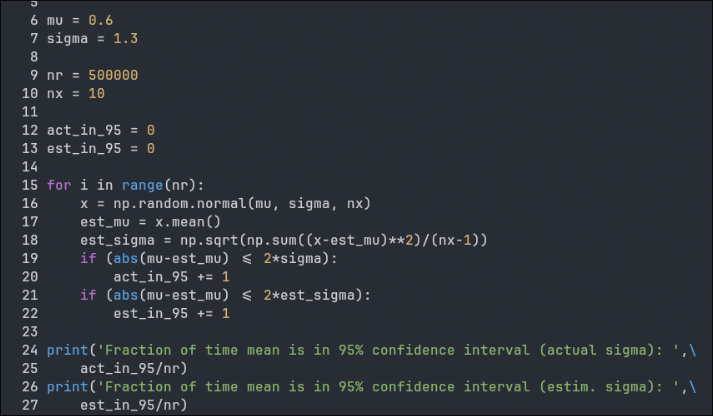
\includegraphics[width=\textwidth]{prob6_code.png}
        \caption{Code to produce the results for this problem}
        \label{fig:prob6_code}
    \end{figure}
    \begin{enumerate}[label=\roman*)]
        \item 1.0
        \item 0.999858
    \end{enumerate}

\section{Characteristic Functions}
    \begin{enumerate}[label=\roman*)]
        \item $E(X) = \mu$
            \begin{proof}
                \begin{align*}
                    E(X) &= \frac{1}{i}\pp{\phi_x}{\xi}\Big|_{\xi = 0}\\
                    &= \left(\mu - \frac{\sigma^2\xi}{i}\right)\exp\left(i\mu\xi -
                    \frac{\sigma^2\xi^2}{2}\right)\Big|_{\xi = 0}\\
                    &= \mu
                \end{align*}
            \end{proof}
        \item $\Var(X) = \sigma^2$
            \begin{proof}
                \begin{align*}
                    \Var(X) &= E(X^2) - (E(X))^2\\
                    &= - \left(\frac{1}{i}\pp{\phi_x}{\xi}\Big|_{\xi = 0}\right)^2
                    - \pptwo{\phi_X}{\xi}\Big|_{\xi = 0}\\
                    &= -\mu^2 - \frac{\partial}{\partial \xi}\left(i\mu -
                    \sigma^2\xi\right)\exp\left(i\mu\xi -
                    \frac{\sigma^2\xi^2}{2}\right)\Big|_{\xi = 0}\\
                    &= -\mu^2 - \left(i\mu -
                    \sigma^2\xi\right)^2\exp\left(i\mu\xi -
                    \frac{\sigma^2\xi^2}{2}\right)\Big|_{\xi = 0} +
                    \sigma^2\exp\left(i\mu\xi -
                    \frac{\sigma^2\xi^2}{2}\right)\Big|_{\xi = 0}\\
                    &= \sigma^2
                \end{align*}
            \end{proof}
    \end{enumerate}

\section{Making an experiment well-posed}
    \begin{enumerate}[label=\roman*)]
        \item No, currently we have no idea of the quantity, nor ratio of coins
        contained in the bin. For example, it could be the case that the bin
        contains 9 type 1 coins for every type 2 coin. If this were the case,
        then this would influence the conditional probability. We also don't
        know if, but would assume that, they are keeping the ratio of the coins
        inside the bins constant, i.e. they are placing the coin back into the
        bag and mixing it up before selecting the next coin. 
        \item In order to make this well-posed, I suggest we include the changes
        to control the number/ratio of each coin in the bin, and make each
        sample identically distributed by placing the coin back into the bin and
        mixing the bin before sampling again. 
    \end{enumerate}
\end{document}
